El presente capítulo proporciona un análisis detallado sobre el
problema de la violencia y las metodologías actuales para su
detección en video, ambos fundamentales para el desarrollo de
esta investigación. Se aborda la clasificación de
los diferentes tipos de violencia y su impacto global, así como
una revisión exhaustiva de los modelos más utilizados en la
literatura para identificar eventos violentos en entornos
audiovisuales.

La Sección \ref{tiposDeViolencia}, establece una categorización de
diversas formas de violencia, la cual destaca su ocurrencia en
diferentes contextos como espacios públicos, entornos
domésticos y situaciones de conflicto. Además, se presentan
estadísticas relevantes para ilustrar la magnitud del problema
a nivel global, con un enfoque particular en América Latina y
sus tendencias recientes.

Por otra parte la Sección \ref{solucionesClásicas}, se listarán las soluciones 
que se están utilizando actualmente para la detección y toma de 
decisiones punitivas de violencia mencionadas en la anterior 
sección.

Por último, la Sección \ref{detecciónIA}, se revisa sistemáticamente 
los enfoques más representativos en la literatura para la
detección de violencia en video. Cada metodología há sdo 
clasificada en función de su fundamento teórico y técnico,
distinguiendo entre modelos basados en extracción manual de
características, redes neuronales convolucionales (CNNs) y
enfoques híbridos. Finalmente, se discute la necesidad de
evaluar diferentes configuraciones de estos modelos para
optimizar su rendimiento en la identificación de incidentes
violentos.


\section{Tipos de Violencia}\label{tiposDeViolencia}
La proliferación de la violencia en todas partes del mundo
constituye un problema social creciente que afecta la convivencia
y el sentido de seguridad entre las personas. Dependiendo de las
características de quienes cometen el acto, la violencia puede
clasificarse en las siguientes categorías \cite{OMS2014}: 
\begin{itemize} 
    \item Autoinfligida (conducta suicida y autolesiones), 
    \item Interpersonal (violencia doméstica, incluyendo a niños, parejas y personas mayores; así como violencia entre personas no relacionadas), 
    \item Colectiva (social, política y económica). 
\end{itemize}

La OMS clasifica los actos violencia según la naturaleza como: 
física, sexual, psicológica, privación y negligencia. 
Con base en datos de 2014, indicó que ``los actos 
repetidos de violencia que van desde la intimidación, el acoso 
sexual y las amenazas hasta la humillación y el menosprecio de 
los trabajadores pueden convertirse en casos muy graves debido 
al efecto acumulativo. En Suecia, se estima que dicho 
comportamiento ha sido un factor en el 10\% al 15\% de los 
suicidios''. En el mismo documento, se menciona que en el año 
2000, hubo alrededor de 199,000 homicidios de jóvenes en todo 
el mundo (9.2 por cada 100,000 habitantes). Es decir, en 
promedio, mueren diariamente 565 niños, adolescentes y adultos 
jóvenes de entre 10 y 29 años como resultado de la violencia 
interpersonal. Las tasas de homicidio varían considerablemente 
según la región, desde 0.9 por cada 100,000 habitantes en 
países de altos ingresos en Europa y algunas partes de Asia y 
el Pacífico hasta 17.6 en África y 36.4 por cada 100,000 en 
América Latina.

Por otro lado, el informe del Fondo Monetario Internacional 
revela un aumento exponencial en la sensación de inseguridad y 
una mayor aceptación de que los crímenes violentos son, 
unánimemente, el problema más importante desde 2020, como 
se muestra en la Figura \ref{fig:percepcion} \cite{Bisca2024}:

\begin{figure}[h!] % Use [H] if you're using the float package to place the image exactly here
    \centering
    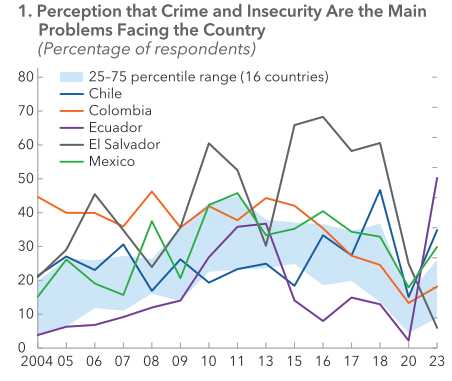
\includegraphics[width=0.7\textwidth]{images/inseguridad2024.png} % Adjust the width and file path
    \caption{Percepción de que la inseguridad es una prioridad \protect\cite{Bisca2024}}
    \label{fig:percepcion}
\end{figure}

La Figura \ref{fig:percepcion} muestra las prioridades con 
respecto al tiempo de la población en diferentes países 
latinoamericanos. La percepción de la prioridad de la violencia 
venía en decadencia desde el 2004, mientras que en los 
últimos 5 años, esta percepción ha mostrado una tendencia 
exponencialmente incremental. En este sentido, en la actualidad, 
la violencia representa la prioridad más importante que 
cualquier gobierno debería abordar. Por esta razón, en este 
proyecto se aborda la solución de este problema a través de la
detección de violencia interpersonal directa, a través del uso 
de inteligencia artificial. 

\section{Soluciones Clásicas}\label{solucionesClásicas}







\section{Detección de violencia a través de IA}\label{detecciónIA}
\thispagestyle{fancy}
En la presente sección, se detallan las arquitecturas y 
procedimientos para comprender mejor tanto el problema
de investigación como la solución propuesta. Entre estos
conocimientos previos, se explican en detalle algunas 
arquitecturas de CNN ampliamente usadas en la clasificación 
de imágenes utilizando ML, así como el procedimiento de 
\textit{Transfer Learning} (TL) y el preprocesamiento de 
entradas. \\

\subsection{\textit{Convolutional Neural Networks} (CNN)}

Las CNN son modelos basados en una arquitectura diseñada
específicamente para el análisis de imágenes, en particular
la clasificación. Estas realizan la tarea de extracción de
características a través de convoluciones. Esto evita la 
pérdida de información y mejora tanto la eficiencia como 
la precisión.\\

Las convoluciones se basan en un procedimiento que extrae
características mediante la aplicación de una pequeña matriz
de transformación cuadrada sobre la imagen original, la cual
retorna una imagen modificada. Estas matrices de transformación
se denominan kernels. La Figura \ref{convolucion} ilustra una
iteración de convolución.\\

\begin{figure}[h!] 
    \includegraphics[width=0.7\textwidth]{images/convolución.png} 
    \centering 
    \caption{Proceso simplificado de una convolución\protect\cite{convoluciones}.} 
    \label{convolucion} 
\end{figure}

Por otro lado, existen otras capas importantes llamadas
\textit{poolings}, como se muestra en la Figura \ref{pooling}.
Estas capas aplican una lógica a un cuadrante de la matriz
resultante de las convoluciones. Esta lógica varía dependiendo
de las necesidades del usuario. La Figura \ref{pooling} muestra una comparación
entre \textit{Max Pooling} y \textit{Average Pooling}, que obtienen
respectivamente los valores máximos y promedios de los cuadrantes
seleccionados para generar un nuevo resultado con menor dimensionalidad.

\begin{figure}[h!] 
    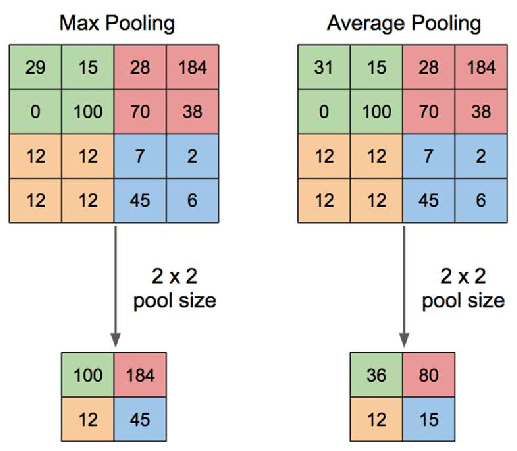
\includegraphics[width=0.6\textwidth]{images/pooling.png} 
    \centering 
    \caption{Proceso simplificado de un pooling \protect\cite{pooling}.} 
    \label{pooling} 
\end{figure}

Las CNN están compuestas por combinaciones repetidas de capas
convolucionales y de \textit{pooling}, finalizando en un conjunto 
de capas densas de neuronas llamadas \textit{Multi Layer 
Perceptron}(MLP), que realiza el procesamiento final de las 
características extraídas. La Figura \ref{CNN} muestra la 
estructura de una CNN. Como se mencionó anteriormente, 
la extracción de características se realiza dentro de la 
propia red neuronal, evitando la pérdida de información que 
se observa en los MLP y dejando únicamente la tarea de 
clasificación a estos últimos.

\begin{figure}[h!] 
    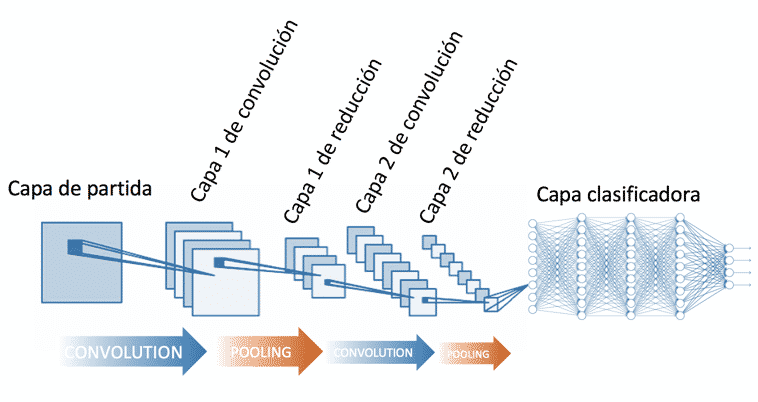
\includegraphics[width=1\textwidth]{images/CNN.png} 
    \centering 
    \caption{Arquitectura de una CNN convencional \protect\cite{CNN-Arquitectura}.} 
    \label{CNN} 
\end{figure}

A continuación, se explican cada una de las arquitecturas que 
son utilizadas en el presente trabajo. 

\section{VGG-19} 

Esta CNN tiene una profundidad de 19 capas y fue
creada por Karen Simonyan y Andrew Zisserman \cite{Simonyan2015}
en la Universidad de Oxford en 2014, y publicada posteriormente
en 2015. Su versión detallada se ilustra en la Figura \ref{VGG19}.
Este modelo fue utilizado para clasificar imágenes en el
\textit{dataset} ImageNet, logrando clasificar hasta 1000 objetos
diferentes. Espera una imagen de entrada de 224x224 píxeles para
su procesamiento. Debido a su profundidad, este modelo es bastante
pesado, llegando a consumir hasta 550 MB de memoria con alrededor
de 143 millones de parámetros. Cabe destacar que el 70\% de estos
parámetros se encuentran entre la última capa convolucional y la
primera capa de clasificación. Con todas estas características,
logró un 90\% de precisión en ImageNet.


\begin{figure}[h!] 
    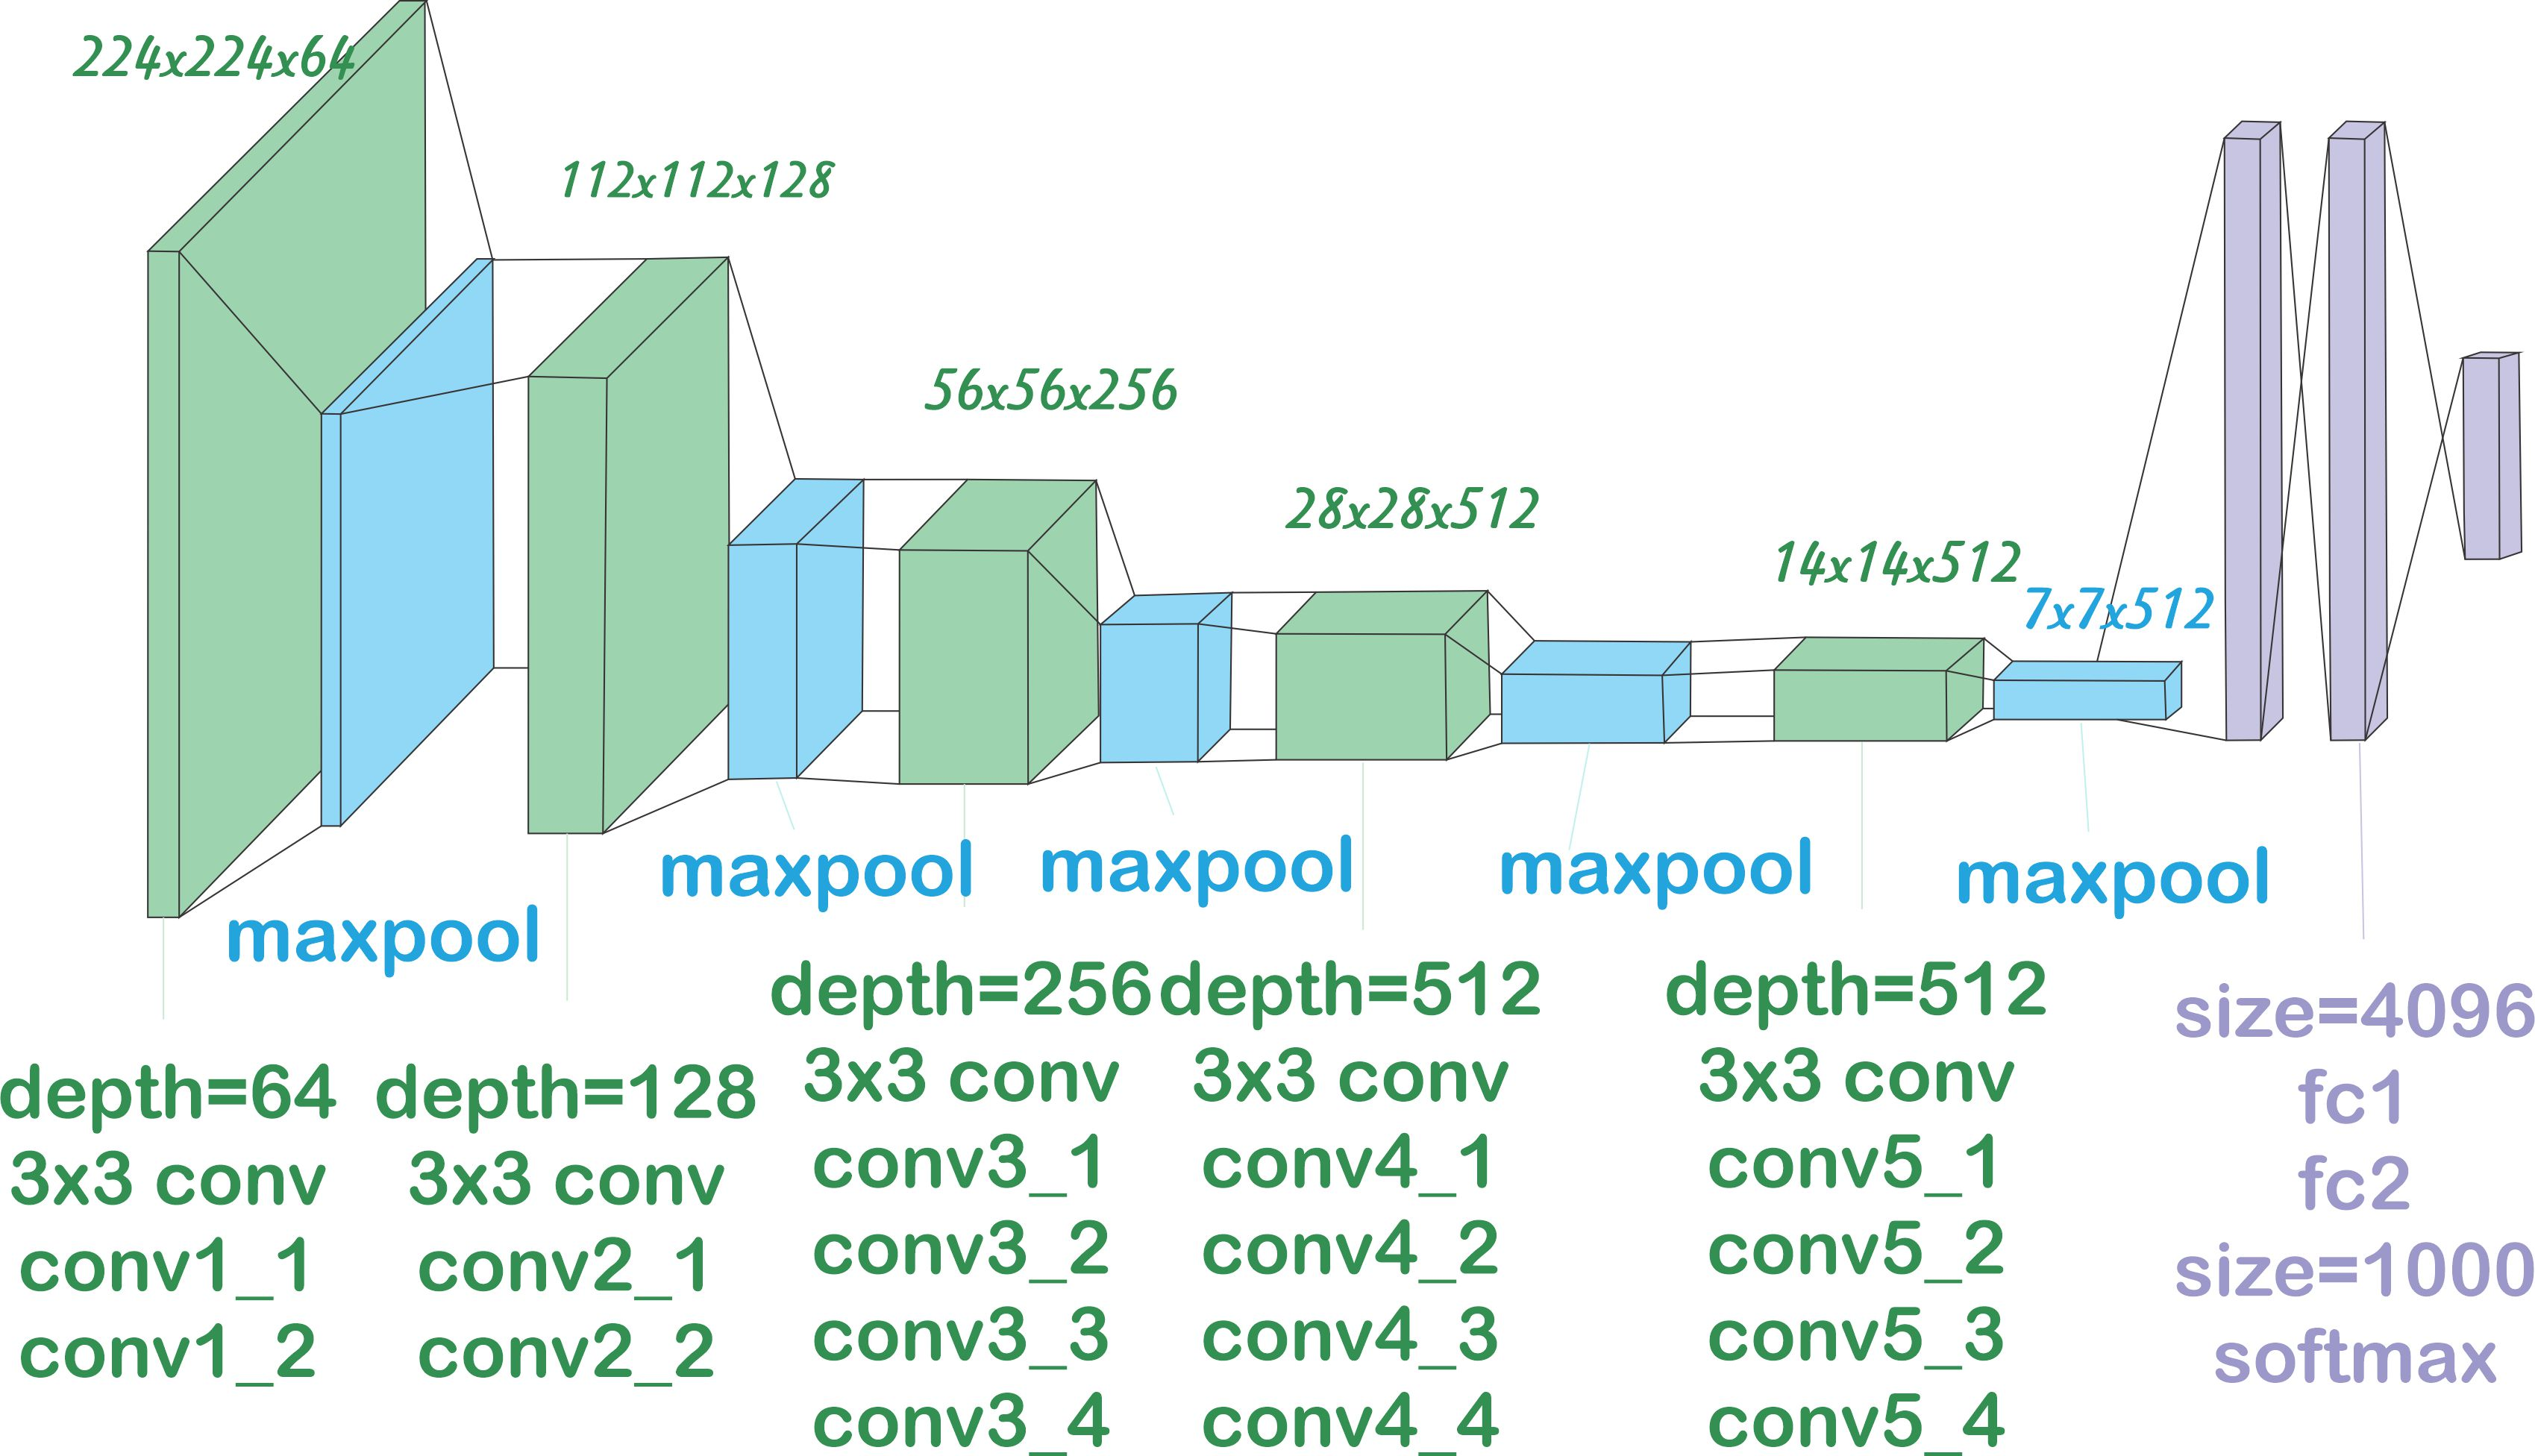
\includegraphics[width=1\textwidth]{images/VGG19.jpeg} 
    \centering 
    \caption{Version simplificada de una VGG19 \protect\cite{modelos}.} 
    \label{VGG19} 
\end{figure}


\section{InceptionV3} \label{sec:inceptionV3}
Aunque VGG19 logró una alta precisión, consumía demasiados
recursos. Por esta razón, Google desarrolló InceptionV3, una
red que prometía resultados similares pero a un menor costo.
Presentado en ``\textit{Going deeper with convolutions}''
\cite{Szegedy2014}, este modelo alcanza un 93.7\% de precisión
en el mismo \textit{dataset}.\

Aunque esta red tiene 50 capas de profundidad (más que VGG19),
tiene menos parámetros entrenables (23.8 millones). Su diseño
propuso que realizar convoluciones unidimensionales en serie
(como se muestra en la Figura \ref{InceptionLayer}) es
equivalente a una convolución bidimensional, evitando el uso
de filtros matriciales. Esto redujo la complejidad de los
modelos CNN convencionales, haciéndolo más liviano en memoria
y mejorando su capacidad de aprendizaje. En total, este modelo
pesa 92 MB—aproximadamente seis veces menos que el anterior.
Requiere imágenes de entrada de 299x299 píxeles, y su
arquitectura se muestra en la Figura \ref{Inceptionv3}.


\begin{figure}[h!] 
    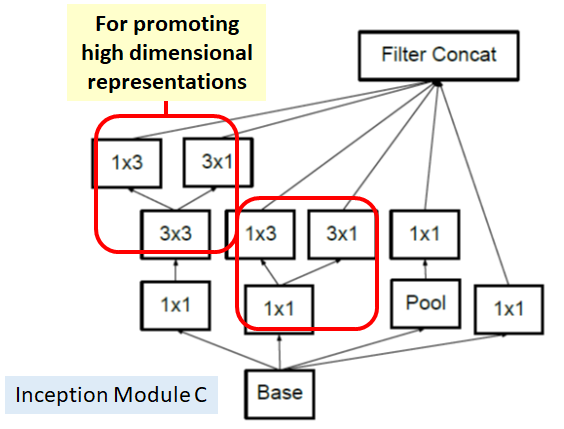
\includegraphics[width=0.8\textwidth]{images/InceptionLayer.png} 
    \centering 
    \caption{Reducción de dimensionalidad de InceptionV3 \protect\cite{modelos}.} 
    \label{InceptionLayer} 
\end{figure}

\begin{figure}[h!] 
    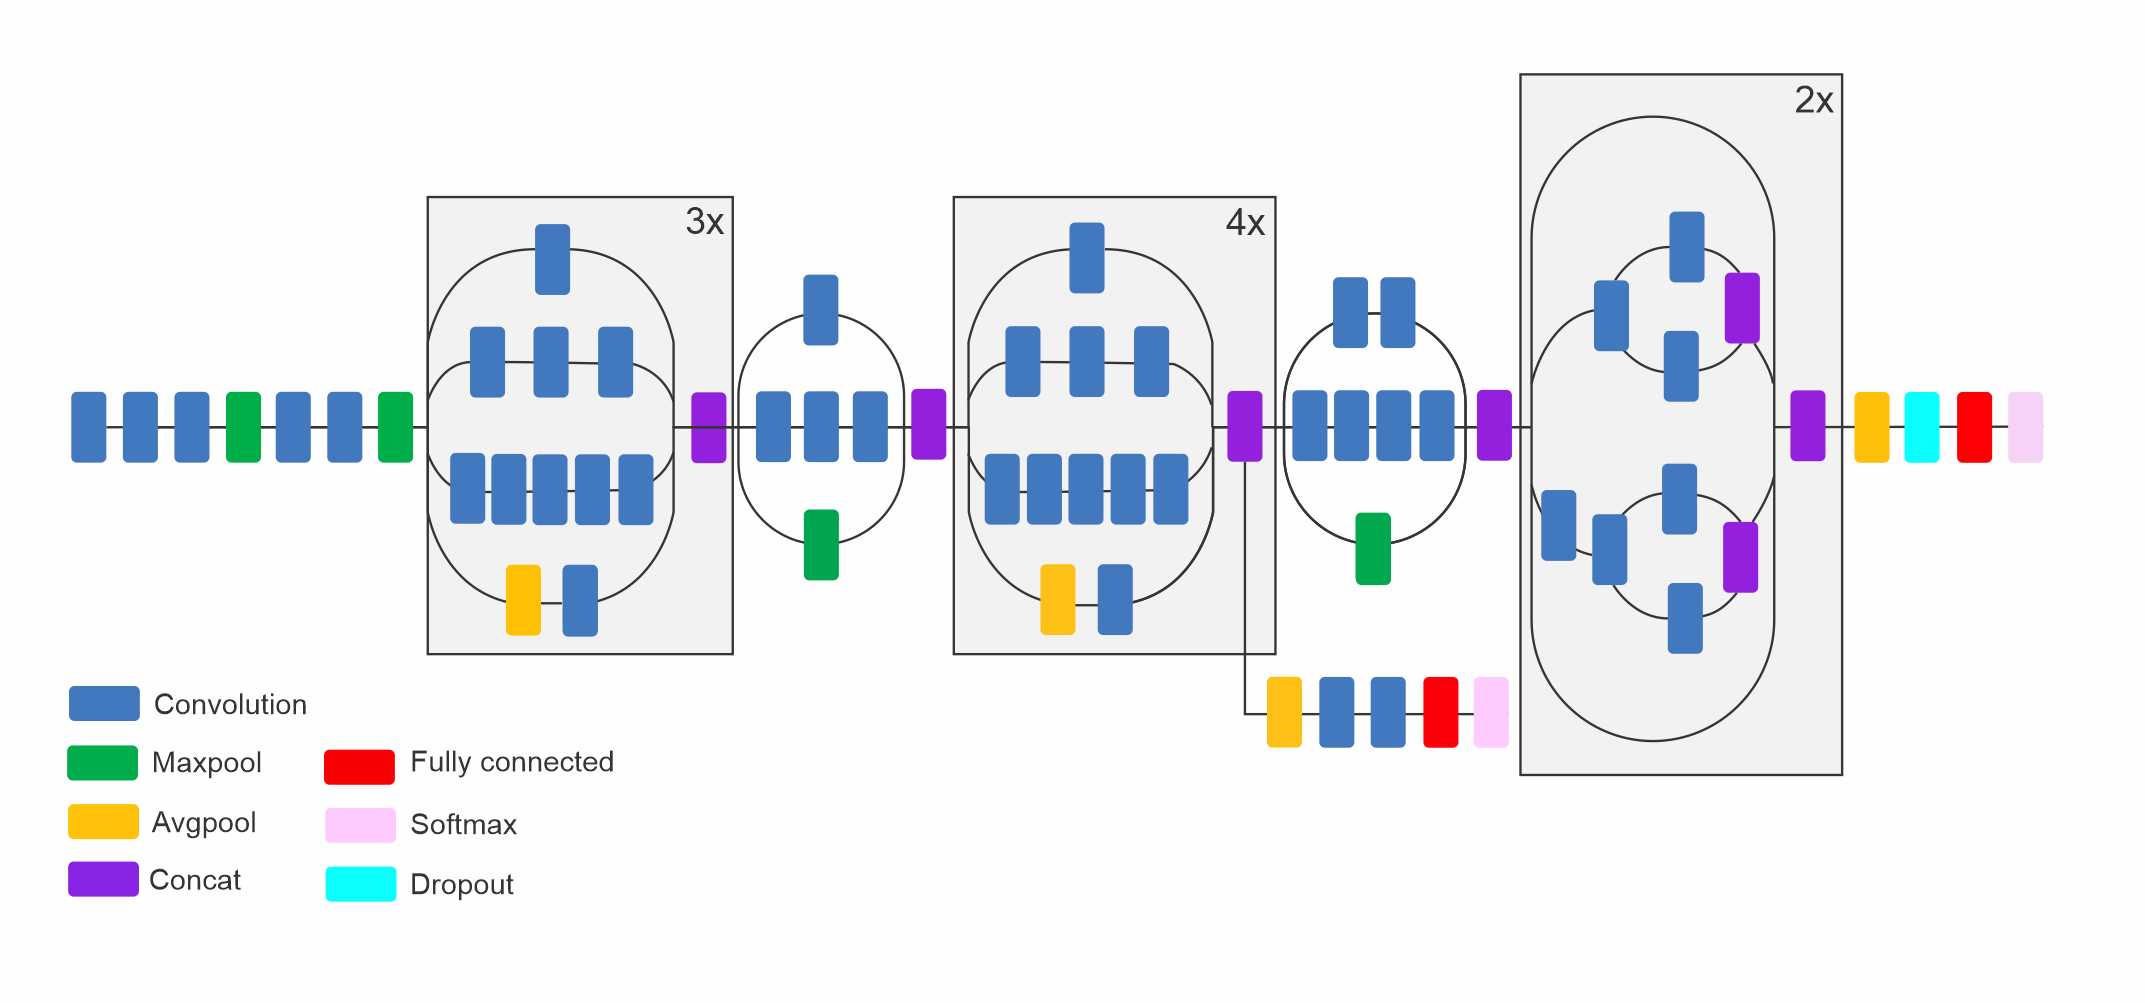
\includegraphics[width=1\textwidth]{images/InceptionV3.png} 
    \centering 
    \caption{Versión simplificada de InceptionV3 \protect\cite{modelos}.} 
    \label{Inceptionv3} 
\end{figure}

\section{ResNet50} 
Creado por Microsoft en 2015, este modelo también cuenta con 50 capas de
profundidad. Emplea una técnica llamada “residual learning”
\cite{He2015}, que consiste en guardar una copia de la salida actual y
sumarla al resultado obtenido de un conjunto de convoluciones (típicamente
cada tres). La Figura \ref{ResNet} ilustra esta modificación y la arquitectura
general del modelo. Este modelo también fue probado en el mismo
\textit{dataset}, obteniendo una precisión del 92.1\%, y el aprendizaje
residual evitó un aumento en la dimensionalidad del modelo.
Contiene aproximadamente 25.6 millones de parámetros y ocupa 98 MB de memoria.

\begin{figure}[h!] 
    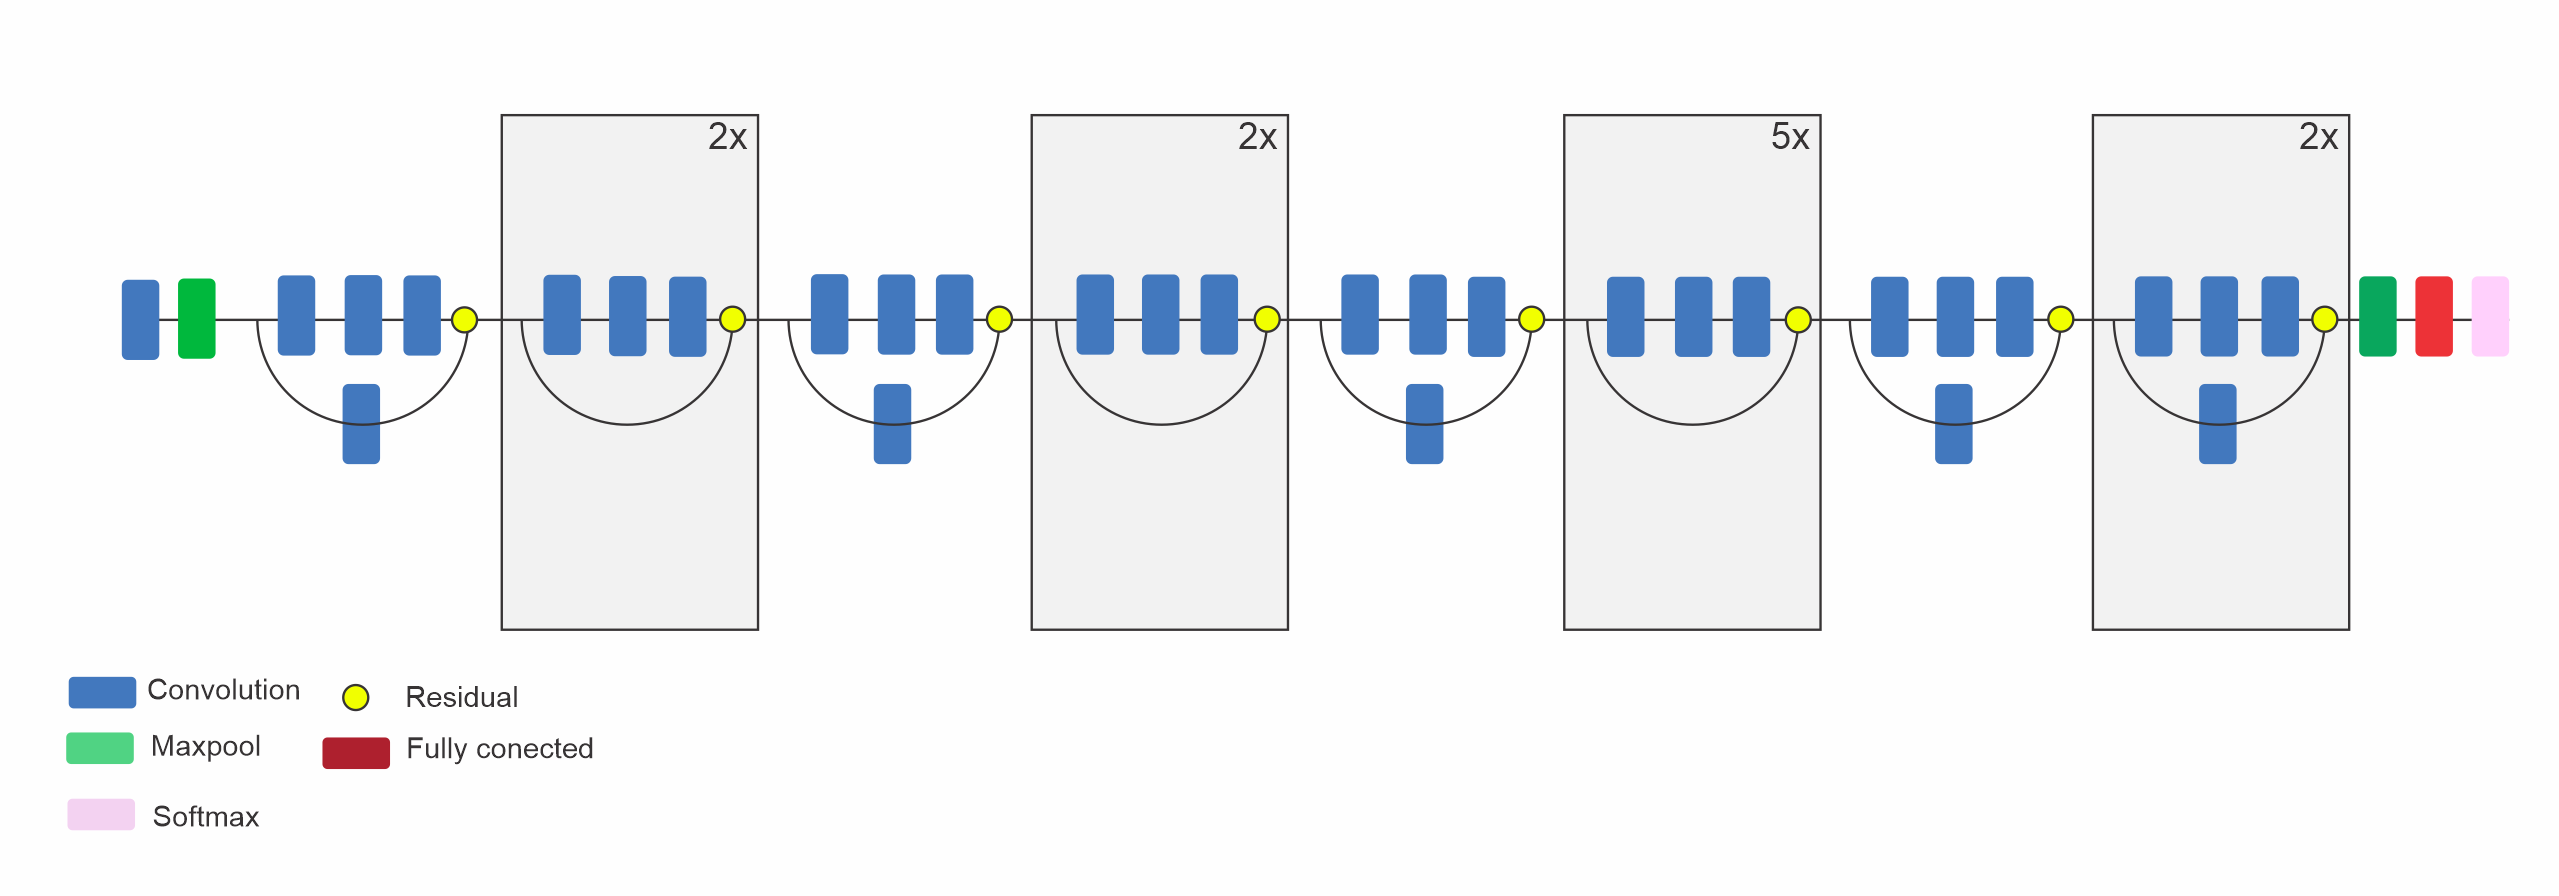
\includegraphics[width=1\textwidth]{images/ResNet.png} 
    \centering 
    \caption{Versión simplificada de ResNet50 \protect\cite{modelos}.} 
    \label{ResNet} 
\end{figure}

\section{EfficientNet} 
``\textit{EfficientNet: Rethinking Model Scaling for 
Convolutional Neural Networks}''\cite{Tan2020} en 2020, 
consiste en 8 implementaciones diferentes (B0 a B7).
La versión más ligera (B0) contiene aproximadamente 5.5 
millones de parámetros y logró un 93\% de precisión en el 
mismo \textit{dataset}. Otras versiones continúan aumentando 
el número de parámetros y la precisión resultante. Comparado 
con los modelos anteriores, EfficientNetB4 con 19.5 millones 
de parámetros alcanza un 96.4\% de precisión, superándolos.
Este modelo optimiza su aprendizaje mediante un algoritmo de 
aproximación que genera parámetros para crear cada uno de 
los ocho modelos. Este algoritmo considera tres factores:

\begin{itemize} 
    \item Profundidad de las capas 
    \item Ancho de las capas (capas múltiples) 
    \item Resolución de la imagen 
\end{itemize} 

La Figura \ref{EfficientNetB0} muestra la estructura de 
EfficientNetB0.

\begin{figure}[h!] 
    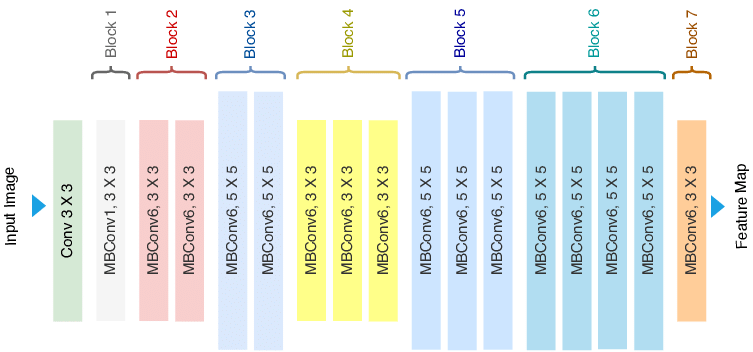
\includegraphics[width=1\textwidth]{images/EfficientNetB0.png} 
    \centering 
    \caption{Versión simplificada de EfficientNetB0 \protect\cite{EfficientNetB0}.} 
    \label{EfficientNetB0} 
\end{figure}

\section{YOLO} 
YOLO (\textit{you only look once}) es una arquitectura que 
permite la ``predicción simultánea de múltiples \textit{bounding boxes} 
y probabilidades de clase para ellas'' \cite{Redmon2015}. 
Este modelo está basado en una CNN convencional, que, a diferencia 
de implementaciones anteriores (R-CNN y FR-CNN), realiza la 
predicción de la caja de enlace internamente, reduciendo la latencia 
y habilitando su uso en tiempo real.\\

Este cálculo se basa en generar cuadrículas o particiones de la 
imagen, dentro de las cuales se inicializa un número predeterminado 
de \textit{bounding boxes} predefinidas (ambos son hiperparámetros de la 
arquitectura). Esto es replicable usando cualquier arquitectura 
CNN como base (por ejemplo, uno de los modelos mencionados previamente), 
solo ajustando la salida y los hiperparámetros en consecuencia. 
Las versiones más recientes logran una mejor detección, módulos de 
atención y otras variaciones que la hacen cada vez más robusta. 
La Figura \ref{YOLO} muestra un ejemplo de la arquitectura del modelo 
YOLOv5.

\begin{figure}[h!] 
    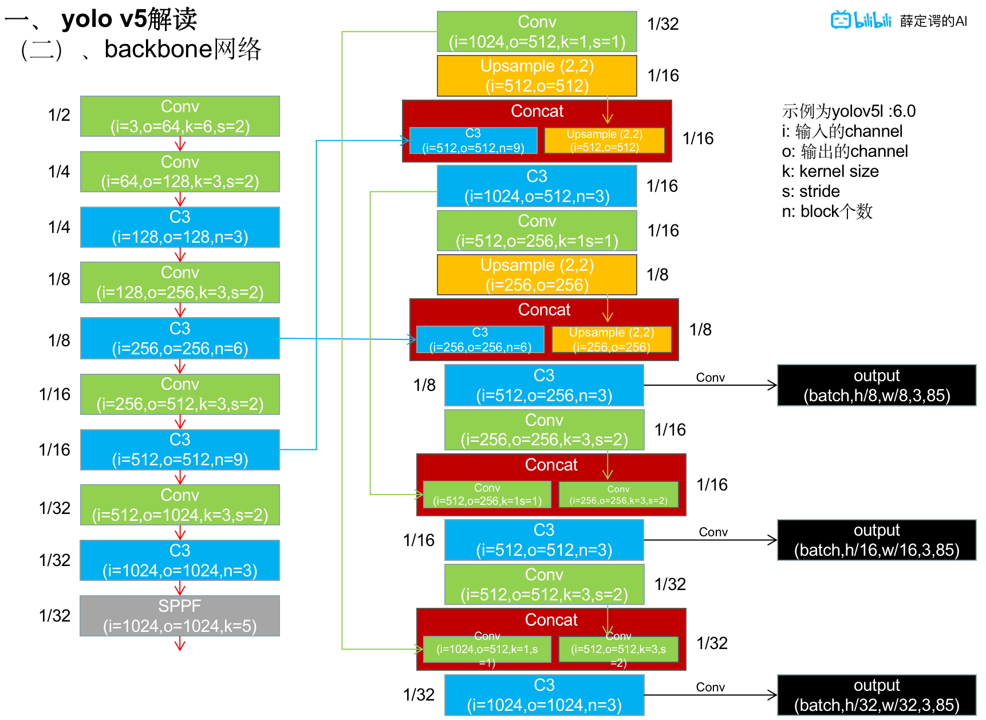
\includegraphics[width=1\textwidth]{images/yolov5.png} 
    \centering 
    \caption{Representación de la arquitectura de YOLOv5\protect\cite{yolov5}.} 
    \label{YOLO} 
\end{figure}

\section{\textit{Long Short-Term Memory} (LSTM)}

Las redes \textit{Long Short-Term Memory} (LSTM) fueron 
desarrolladas como una extensión de las redes neuronales 
recurrentes (RNN) con el propósito de superar la dificultad 
de aprender dependencias a largo plazo en secuencias
\cite{hochreiter1997lstm}. Las 
RNN tradicionales tienden a sufrir del problema del 
desvanecimiento o explosión del gradiente durante el 
proceso de entrenamiento, lo que limita su capacidad 
para capturar relaciones temporales distantes. Las LSTM 
abordan esta limitación mediante la incorporación de una 
memoria interna controlada por compuertas, lo que permite 
conservar información relevante a lo largo del tiempo.

La arquitectura de las LSTM se basa en una celda de memoria 
capaz de mantener su estado a lo largo de múltiples pasos 
temporales. Esta celda está regulada por tres compuertas 
fundamentales: la compuerta de entrada, que controla qué 
nueva información se almacena en la celda; la compuerta 
de olvido, que decide qué información debe eliminarse 
del estado anterior; y la compuerta de salida, que 
determina qué parte del contenido de la celda se utiliza 
como salida. Estas compuertas permiten que la red aprenda a 
retener o descartar información de manera adaptativa, mejorando 
significativamente el aprendizaje de secuencias largas.

Gracias a esta estructura, las LSTM han demostrado un 
rendimiento notable en una amplia gama de tareas secuenciales 
donde el contexto temporal es esencial. Aplicaciones como 
el modelado del lenguaje natural, la traducción automática, 
el reconocimiento de voz y el análisis de series temporales 
se han beneficiado enormemente de su capacidad para capturar 
dependencias a largo plazo. En consecuencia, las LSTM se han 
convertido en una arquitectura fundamental dentro del campo 
del aprendizaje profundo secuencial.La arquitectura de este modelo se puede ver en la imagen 
\ref{lstm}:

\begin{figure}[h!] 
    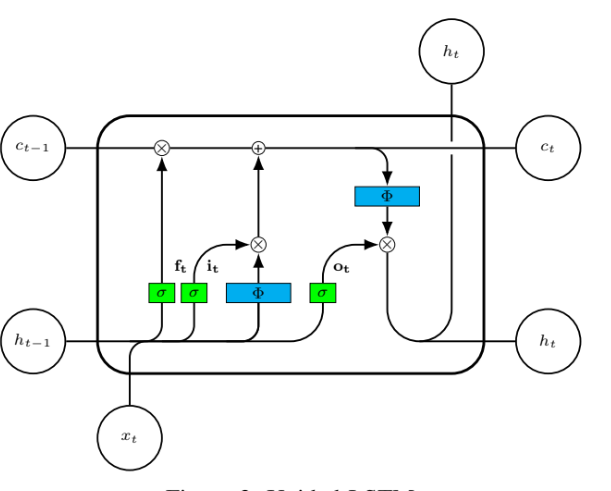
\includegraphics[width=1\textwidth]{images/lstm.png} 
    \centering 
    \caption{Representación de la arquitectura de LSTM\protect\cite{datascientest2024lstm}.} 
    \label{lstm} 
\end{figure}


\subsection{\textit{Transfer Learning}}
Según Muhamad Yani \cite{Yani2019}, 
\textit{Transfer Learning (TL)} se define como ``el proceso de 
transferir el conocimiento de un entrenamiento previo para ser 
utilizado en un nuevo modelo con el fin de reducir el tiempo de 
aprendizaje''. Este proceso puede ser observado en la Figura 
\ref{transfer-learning}.\\

\begin{figure}[h!]
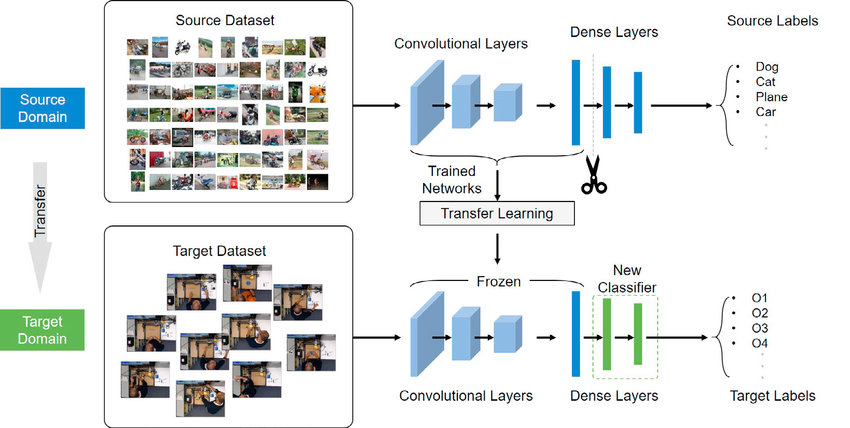
\includegraphics[width=1\textwidth]{images/transfer-learning.png}
\centering
\caption{Comparativa entre un entrenamiento normal y por TL\protect\cite{transfer-learning}.}
\label{transfer-learning}
\end{figure}
TL difiere del proceso de entrenamiento convencional de una 
red en que no es necesario entrenarla con un gran conjunto de 
datos. A diferencia del proceso tradicional, las capas iniciales 
del modelo (en nuestro caso, las capas convolucionales) están 
congeladas. Estas capas contienen todo el conocimiento pre-aprendido 
del conjunto de datos con el cual el modelo fue originalmente entrenado. 
Una vez obtenidas esas capas, se agregan nuevas capas densas (similares 
a las de un MLP) que sirven como clasificadores para nuestro propósito 
específico. Gracias a esto, solo las capas finales necesitan ser entrenadas, 
lo que requiere menos datos y generalmente resulta en predicciones precisas. 
Este tipo de entrenamiento se llama ``\textit{fine-tuning}'', lo que permite 
que la red ajuste el aprendizaje previo para predecir en función de un conjunto 
de datos diferente al que fue entrenada originalmente, ahorrando tiempo y 
mejorando la precisión.

\subsection{Preprocesamiento de Entradas}
Ahora que entendemos cómo funcionan estos modelos en general, 
necesitamos observar las características requeridas de las 
entradas para que el modelo aprenda de manera efectiva.

\subsubsection{Tamaño de la Entrada}
Considerando solo las diferentes CNN, cada modelo espera una 
matriz de entrada (imagen) de un tamaño específico. En las 
implementaciones actuales, se usan comúnmente tensores para 
referirse a un \textit{batch} (conjunto) de imágenes. La 
representación es la siguiente:

$$(batch, channels, m, n), donde:$$
\begin{itemize}
    \item batch: Número de imágenes que se ingresan a la vez.
    \item channels: Número de canales de la imagen (para imágenes a color, hay 3 canales que representan RGB, mientras que las imágenes en escala de grises tienen solo 1 canal).
    \item m \& n: Dimensiones de la imagen. Estos valores dependen de la arquitectura del modelo, ya que cada capa realizará operaciones que reducen la dimensionalidad de la imagen. Esto varía según la implementación debido a las diversas configuraciones posibles para cada matriz convolucional y operación de pooling.
\end{itemize}

\subsubsection{\textit{One Hot Encoder}}
Este es un tipo de representación que consiste en crear una 
matriz identidad de tamaño $n \times n$, donde $n$ es 
el número de \textit{etiquetas}. La codificación de cada 
etiqueta puede tomarse como una de las filas de la matriz. 
Así, podemos representar la codificación de un objeto de 
la clase j entre n clases como:

$$OneHotEncoder(i,j,n)= [a_1,a_2, .. a_n], donde: $$
\begin{equation*}
a_{i,j}=
\begin{cases}
1 & \text{si j = i}\\
0 &  \text{otherwise}
\end{cases}
\end{equation*}
Este tipo de codificación tiene la ventaja de evitar 
relaciones entre etiquetas, y permite una clasificación 
sencilla al comparar resultados. En el lado negativo, 
puede llevar a una alta dimensionalidad cuando hay muchas 
\textit{etiquetas}.

\subsection{\textit{Overfitting}}
El proceso de aprendizaje de los modelos se basa en la retroalimentación 
obtenida a través de la retropropagación mencionada anteriormente. 
Una vez que se actualizan los pesos de cada neurona utilizando el 
gradiente resultante, se puede decir que el modelo ha aprendido 
a clasificar esa imagen específica. Sin embargo, este gradiente 
puede desvanecerse debido a la profundidad de la arquitectura, 
las funciones de activación u otras razones. Este gradiente 
desvanecido impide que el modelo siga aprendiendo del 
conjunto de datos, lo que lo hace inutilizable para aplicaciones 
del mundo real. Algunas estrategias utilizadas para abordar 
esto son:

\begin{itemize}
    \item {\textit{Data Augmentation}: Expansión del conjunto 
    de datos original utilizando rotaciones, escalados, recortes, 
    volteos, etc. Esto hace que el modelo sea más resistente 
    a los cambios en la posición o orientación del objeto en la imagen.}
    \item {\textit{Batch Normalization}: Reescalado de los datos 
    de entrada a diferentes rangos relativos a una escala común, 
    generando una distribución de datos más manejable.}
    \item {\textit{Dropout}: Desactivación aleatoria de un 
    porcentaje de neuronas artificiales en una capa. Esto 
    impide que cada neurona dependa de las desactivadas, 
    mejorando generalmente el rendimiento.}
\end{itemize}

Este capítulo presentó los conocimientos previos que 
ayudarán a los lectores a comprender mejor la metodología 
que se introducirá más adelante particularmente las arquitecturas de 
los modelos que se revisarán, utilizarán y compararán para 
lograr los mejores resultados posibles en la detección y clasificación 
de imágenes de peces dentro de la fauna marina peruana.



\subsection{\textit{Pipelines} actuales para la clasificacion de violencia}

La literatura actual muestra un creciente interés en la 
detección automática de violencia en videos mediante la 
combinación de redes convolucionales (CNN) y redes de 
memoria a largo plazo (LSTM). Las CNN se utilizan para extraer 
características espaciales relevantes de los fotogramas, 
permitiendo identificar patrones visuales y contextos que podrían 
indicar situaciones violentas. Posteriormente, estas 
características son procesadas por las LSTM, las cuales se 
encargan de capturar la dinámica temporal y las dependencias 
de largo plazo entre los fotogramas, mejorando la capacidad 
de detectar eventos violentos que se desarrollan a lo largo 
del tiempo.\\

En diversos estudios se ha demostrado que la integración 
de ambas arquitecturas permite explotar de forma sinérgica 
las ventajas de cada una: las CNN fortalecen la comprensión 
del contenido visual a nivel de detalle y textura, mientras 
que las LSTM aportan una perspectiva temporal que es crucial 
para identificar patrones de comportamiento complejos y 
secuenciales propios de la violencia. Este tipo de 
\textit{pipeline} ha sido evaluado en diferentes escenarios, 
incluyendo videos de vigilancia y grabaciones deportivas, 
logrando así mejores tasas de detección en comparación con 
métodos que utilizan únicamente análisis espacial o temporal 
de manera aislada.\\

Un claro ejemplo de lo mencionado anteriormente, 
es el artículo de Jeff Donahue, \textit{et al.}
\cite{Donahue2016}. Su investigación se centra en el 
desafío de trabajar con datos visuales que contienen 
información espacial y temporal. La idea central es 
integrar ambas arquitecturas en un único sistema 
end-to-end: las CNNs se encargan de extraer 
representaciones ricas de contenido visual, y las 
LSTMs modelan la dinámica secuencial, permitiendo 
aplicaciones en reconocimiento de actividades en video y 
generación de descripciones de imágenes. \\

Entre sus principales contribuciones, este trabajo 
logró sentar las bases las bases en la integración de 
arquitecturas visuales y secuenciales. Su enfoque ha 
influido en numerosos trabajos posteriores en áreas como 
la descripción automática de videos, el análisis de 
secuencias complejas y el desarrollo de modelos más 
integrados para tareas multimodales.\\

Utilizando esta lógica, el trabajo de Orozco, \textit{et al.}\cite{Orozco2021} el cual 
destaca la efectividad de estas estrategias al combinar 
etapas de preprocesamiento, extracción de características 
espaciales mediante CNN, y análisis secuencial temporal con 
LSTM. Asimismo, se discuten los desafíos asociados a la 
variabilidad de escenarios y la detección en tiempo real, 
aspectos que continúan motivando la investigación y 
optimización de estos sistemas. Como resultado final de su 
experimentación, los autores lograron un F1-score de 91\% 
lo cual indica que fue \textit{pipeline} robusto el 
problema que intentó resolver basado en la clasificación de 
acciones humanas basado en videos. Los pipelines híbridos 
basados en CNN y LSTM representan una tendencia robusta en 
el campo de la detección de violencia, contribuyendo 
significativamente a la mejora en la precisión y eficiencia 
de los sistemas de análisis de video.\\

Otro artículo que también utiliza esta misma lógica es el de
Swathikiran Sudhakaran and Oswald Lanz\cite{Sudhakaran2017}. Su objetivo consistió 
en el mismo del presente trabajo, la detección de violencia. 
Para ello, se utilizó el \textit{dataset} de Hockey Fights, 
el cuál contiene videos de eventos violentos en partidos de 
hockey. Este \textit{dataset} es bastante usado como \textit{benchmark} 
y consiste de un conjunto de imágenes etiquetadas de manera 
homogenea. La variación más significativa que realizaron fue el 
uso de celdas convLSTM en vez de LSTM regulares para poder 
obtener un \textit{accuracy} más elevado. Con su \textit{pipeline} 
lograron obtener una \textit{accuracy} de 97\%, generando un 
nuevo record para este \textit{benchmark} y marcando un nuevo 
estado del arte. \\


De la misma manera y utilizando el mismo \textit{dataset} de 
Hockey Fights, se encuentra el trabajo de Al-Maamoon R. Abdali 
y Rana F. Al-Tuma\cite{Abdali2019}. Ellos se basaron en el 
trabajo anteriormente mencionado para su implementación. 
Para ello, utilizaron la misma configuración del 
\textit{pipeline} pero incluyeron capas 
conv3d y 40 celdas para el aprendizaje de la LSTM sin ser 
convolucionales. Utilizando aquella configuración logrando 
obtener un \textit{accuracy} de 96.33\% 
pero al mismo tiempo obteniendo una mejora de 4 veces en la 
velocidad (representado en el número de fps), representando 
una mejora del estado del arte en su tiempo al mantener el 
mismo nivel de \textit{accuracy} pero mejorando el 
\textit{performance}.\\


El último artículo a revisar es el de Patel Mann 
\cite{Mann2021}. En su trabajo utilizó Resnet50, InceptionV3 
y VGG19 como extractores de características. En cambio, 
utilizaron solo una celda LSTM para la clasificación y como 
resultados obtuvieron 90\% de precisión para 
el dataset de Hockey fights, representando una disminución a 
comparación de los anteriores trabajos, aunque permitió optimizar 
el uso de memoria sin perder drásticamente el \textit{performance} 
de todo el \textit{pipeline}.\\

Como se puede ver, el \textit{pipeline} CNN-LSTM propuesto ha 
sido utilizado a lo largo de los últimos años para resolver 
problemas similares e iguales al nuestro. En ese sentido nos hace 
sentido tratar de extender la aplicación de este y optimizarlo 
para tratar de ver como es que diferentes configuraciones del 
mismo permiten mejorar ya sea el \textit{performance} o el 
\textit{accuracy} de la propuesta.

